\documentclass[30pt, french]{tccv}
\usepackage[hmargin=0.2cm,vmargin=0cm]{geometry}
\usepackage{amsfonts} 								% for the \checkmark command 
\usepackage[framemethod=TikZ]{mdframed}						% For box around text
\usepackage[overlay,absolute]{textpos}						% For Textblock
\setlength{\TPHorizModule}{1cm}
\setlength{\TPVertModule}{1cm}
\usepackage{fontspec}								% For extended fonts
\usepackage{enumitem}								% For aptitudes enumeration 








\begin{document}
\begin{upshape}
\fontsize{9pt}{1em}\color{text}\selectfont



%%%%%%%%%%%%%%%%%%%%%%%%%%%%%%%%%%%%%%%%%%%%%%%%%%%%%%%%%%%%%%%%%%%%%%%%%%%%%%%%%%%%%%%%%%%%%%%%%%%%%%%%%%%%%%%%%%%%%%%%%%%%%%%%%%%%%%%%%%%%%%%%%%%%%%%%%%%%%%%%%%%%%%
%
%			0/ HEADER
%
%%%%%%%%%%%%%%%%%%%%%%%%%%%%%%%%%%%%%%%%%%%%%%%%%%%%%%%%%%%%%%%%%%%%%%%%%%%%%%%%%%%%%%%%%%%%%%%%%%%%%%%%%%%%%%%%%%%%%%%%%%%%%%%%%%%%%%%%%%%%%%%%%%%%%%%%%%%%%%%%%%%%%%




\begin{textblock}{6.5}( 0.5 , 0.7 )
\personal
    [Italo - chilienne]
    {\specialcell{49 Quai de la Prévalaye \\ 35000 }}
    {+33 07 83 88 33 32}
    {r.sanhuezarepetto@gmail.com}
\end{textblock}

\begin{textblock}{21}(0.5,1)
     \centering{\headerfirstnamestyle{Roc\'io}   \headerlastnamestyle{Sanhueza}}
\end{textblock}

\begin{textblock}{21}(17.2,0.6)
		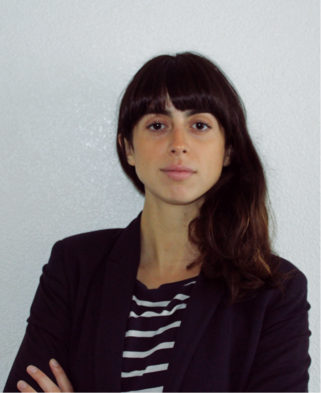
\includegraphics[width=3cm]{../Figure/Rocio3.png}
\end{textblock}  



\begin{textblock}{21}(0,2.3)

\begin{center}
	{\fontsize{20pt}{5em}\scshape\bfseries Serveuse polyvalente \\} 

	\vspace{5pt}
	
	{\fontsize{15pt}{3.5em}\color{text}\bodyfontlight\upshape \\}
\end{center}
\end{textblock}  





%%%%%%%%%%%%%%%%%%%%%%%%%%%%%%%%%%%%%%%%%%%%%%%%%%%%%%%%%%%%%%%%%%%%%%%%%%%%%%%%%%%%%%%%%%%%%%%%%%%%%%%%%%%%%%%%%%%%%%%%%%%%%%%%%%%%%%%%%%%%%%%%%%%%%%%%%%%%%%%%%%%%%%
%
%			1/ EDUCATION
%
%%%%%%%%%%%%%%%%%%%%%%%%%%%%%%%%%%%%%%%%%%%%%%%%%%%%%%%%%%%%%%%%%%%%%%%%%%%%%%%%%%%%%%%%%%%%%%%%%%%%%%%%%%%%%%%%%%%%%%%%%%%%%%%%%%%%%%%%%%%%%%%%%%%%%%%%%%%%%%%%%%%%%%




\begin{rounded_frame}{Éducation}{6.5}{0.5}{3.7}{}
\begin{yearlist}

\vspace{0.5cm}
\item[Master 1 Science politique]{2015 -- 2016}
     {Université de Rennes 1}
     {Enseignements suivis: pensée politique contemporaine, 
     régimes contemporaines, sociologie de la communication, pensée sociologique, 
     Appro\-ches de l'Union Européen, Grands dossiers de\- l'ad\-mi\-ni\-stra\-tion.}



\vspace{0.5cm}
\item[Diplôme en Communication sociale et journalisme (Bac+5)]{2008 -- 2013}
     {Universidad de Santiago de Chile}
     {Spécialité: politique
     }

 \vspace{0.5cm}    
\item[Échange universitaire -- journalisme]{2011 -- 2011}
     {Universidade Estadual Pau\-li\-sta}
     {Enseignements suivis: réalité socio - é\-co\-no\-mi\-que et politique brésilienne. \\
     Langue portugaise: littérature, sémiotique, stra\-té\-gies de communication publique}


\end{yearlist}
\end{rounded_frame}



%%%%%%%%%%%%%%%%%%%%%%%%%%%%%%%%%%%%%%%%%%%%%%%%%%%%%%%%%%%%%%%%%%%%%%%%%%%%%%%%%%%%%%%%%%%%%%%%%%%%%%%%%%%%%%%%%%%%%%%%%%%%%%%%%%%%%%%%%%%%%%%%%%%%%%%%%%%%%%%%%%%%%%
%
%			2/ COMPETENCE
%
%%%%%%%%%%%%%%%%%%%%%%%%%%%%%%%%%%%%%%%%%%%%%%%%%%%%%%%%%%%%%%%%%%%%%%%%%%%%%%%%%%%%%%%%%%%%%%%%%%%%%%%%%%%%%%%%%%%%%%%%%%%%%%%%%%%%%%%%%%%%%%%%%%%%%%%%%%%%%%%%%%%%%%


\begin{rounded_frame}{Compétences linguistiques}{6.5}{0.5}{16.5}{}

\begin{factlist}
\item{Espagnol} {Langue maternelle}	
\item{Français} {Courant}	
\item{Anglais}  {Niveau B2}	
\item{Portugais}{Niveau B2}
\end{factlist}

\vspace{0.5cm}
\section{Logiciels}
Environnement PC et Linux, \\
Pack office et Libre office,
Adobe Photoshop, Premiere, \\
Gimp,
\LaTeX.

\vspace{0.5cm}
\section{Aptitudes}
\begin{itemize}[leftmargin=13pt]
  \setlength\itemsep{-3pt} 

  \cvitem[\checkmark]  Faculté d'adaptation et d'organisation
  \cvitem[\checkmark]  Riguereuse
  \cvitem[\checkmark]  Dynamique et motivé
  \cvitem[\checkmark]  Maîtrise de plusiers langues
\end{itemize}

\vspace{0.3cm}

\end{rounded_frame}




%%%%%%%%%%%%%%%%%%%%%%%%%%%%%%%%%%%%%%%%%%%%%%%%%%%%%%%%%%%%%%%%%%%%%%%%%%%%%%%%%%%%%%%%%%%%%%%%%%%%%%%%%%%%%%%%%%%%%%%%%%%%%%%%%%%%%%%%%%%%%%%%%%%%%%%%%%%%%%%%%%%%%%
%
%			3/ EXPERIENCE
%
%%%%%%%%%%%%%%%%%%%%%%%%%%%%%%%%%%%%%%%%%%%%%%%%%%%%%%%%%%%%%%%%%%%%%%%%%%%%%%%%%%%%%%%%%%%%%%%%%%%%%%%%%%%%%%%%%%%%%%%%%%%%%%%%%%%%%%%%%%%%%%%%%%%%%%%%%%%%%%%%%%%%%%


\begin{flat_frame}{Expérience Professionnelle}{13.3}{7.3}{3.7}{}
\begin{eventlist}


    
    
    
%\setlength{\parskip}{0pt}
\item{Déc 2016 -- Juin 2017}
     {Direction Éducation Enfance, Rennes}
     {Animatrice périscolaire}
     \fontsize{9pt}{1em}\color{text}\bodyfontlight\upshape\selectfont
    
    \begin{itemize}
      \cvitem[\checkmark] Accueillir les enfants et les familles                      
      \cvitem[\checkmark] Encadrer par l’animation un groupe d’enfants
      \cvitem[\checkmark] Animer, construire et maintenir la dynamique de groupe               
      \cvitem[\checkmark] Assurer le développement physique, psychologique et affectif de l’enfant                                            
    \end{itemize}     




\setlength{\parskip}{0pt}    
\item{Sept. 2016 -- Juin 2017 }     
  {Agence Zouzous Rennais, Rennes}     
  {Babysitting}
     \fontsize{9pt}{1em}\color{text}\bodyfontlight\upshape\selectfont

\begin{itemize}
      \cvitem[\checkmark]  Prendre en charge l’enfant à son domicile                                    
      \cvitem[\checkmark]  Animer des activités ludiques ou l’aider lors d’activités d’éveil et d’apprentissage                                            
      \cvitem[\checkmark]  Assurer un suivi des devoirs
      \cvitem[\checkmark]  Préparer et donner un repas

\end{itemize}       





  
\setlength{\parskip}{0pt}
\item{Mai. 2014 -- Mars 2015 }     
  {Sénat du Chili, Santiago, Chili}     
  {Attachée et cordinatrice de presse}
  \fontsize{9pt}{1em}\color{text}\bodyfontlight\upshape\selectfont

  
\begin{itemize}
      \cvitem[\checkmark] Élaboration et mise en œuvre des stratégies de communication conjointement avec la Chef de cabinet
      \cvitem[\checkmark] Rédaction des articles, communiqués et dossiers de presse
      \cvitem[\checkmark] Suivi et relances du contenu envoyé à la presse
      \cvitem[\checkmark] Analyse et suivi des contenus des médias à fin de faciliter l'Identification des thèmes pertinents
\end{itemize}        




\setlength{\parskip}{0pt}
\item{Avril 2013 -- Déc 2014 }     
  {Aluro 35, Santiago, Chili}     
  {Productrice générale}
\fontsize{9pt}{1em}\color{text}\bodyfontlight\upshape\selectfont

    
\begin{itemize}
      \cvitem[\checkmark] Génération de rapports avec la chaîne et négociation du budget                   
      \cvitem[\checkmark] Préparation des lieux de tournage, mobilisation et interviews. Aide à la préparation du contenu des entretiens   
      \cvitem[\checkmark] Administration des réseaux sociaux et animation des communautés (Facebook, Twitter, Instagram)                                                                    
      \cvitem[\checkmark] Création de dossiers de presse pour les lancements du programme      
\end{itemize}      
  


\setlength{\parskip}{0pt}
\item{\color{text} Juin 2013 -- Fév.2014}
     {Capperi, Santiago, Chili}
     {Serveuse restaurant Italian}
     \fontsize{9pt}{1em}\color{text}\bodyfontlight\upshape\selectfont

    \begin{itemize}
      \cvitem[\checkmark] Accueillir, installer et prendre les commandes des clients
      \cvitem[\checkmark] Suivre la sortie des plats de la cuisine selon les bons de commande
      \cvitem[\checkmark] Débarrasser les tables et les (re)dresser
      \cvitem[\checkmark] Présenter l’addition à la demande du client
      
    \end{itemize}       
  
  
\end{eventlist}
\end{flat_frame}








\end{upshape}
\end{document}
